\newpage
\subsubsection{Biểu đồ use case tổng}
\begin{figure}[H]
    \centering
     \includesvg[width=1\textwidth]{Dg_UC/General.svg}
    \vspace{0.5cm}
    \caption{Biểu đồ use case tổng}
    \label{fig:enter-label}
\end{figure}
%-------------------------------------------------------------------
\subsubsection{Quản lý tài khoản}
\subsubsubsection{Biểu đồ use case}
\begin{figure}[H]
    \centering
     \includesvg[width=1\textwidth]{Dg_UC/ManageAccount.svg}
    \vspace{0.5cm}
    \caption{Biểu đồ use case cho Quản lý tài khoản}
    \label{fig:enter-label}
\end{figure}

\subsubsubsection{Use case scenario}
\textbf{Đăng ký tài khoản mới}
\begin{table}[H]
	\centering
	\begin{tabular}{|l|l|l|l|} 
		\hline Use case name: & \multicolumn{3}{|l|}{Đăng ký tài khoản mới} \\ 
		\hline Created by: & Nguyễn Đức An & Last updated by: & Nguyễn Đức An \\ 
		\hline Date created: & $19 / 10 / 2024$ & Date last updated: & $19 / 10 / 2024$\\ 
		\hline Actors: & \multicolumn{3}{|l|}{ Nhân viên (gồm nhân viên chăm sóc khách hàng, quản trị viên) } \\ 
		\hline Description: & \multicolumn{3}{|p{12cm}|}{ Cho phép nhân viên đăng ký tài khoản mới. } \\ 
		\hline Trigger: & \multicolumn{3}{|p{12cm}|}{ Chọn vào nút "Đăng ký mới". } \\ 
		\hline Preconditions: & \multicolumn{3}{|p{12cm}|}{ Nhân viên cần chuẩn bị email doanh nghiệp. } \\ 
		\hline Postconditions: & \multicolumn{3}{|p{12cm}|}{ Đăng ký thành công tài khoản. } \\ 
		\hline Normal Flows: & \multicolumn{3}{|p{12cm}|}{
			1. Nhân viên điền đầy đủ thông tin trong trang đăng ký. \newline
			2. Nhân viên đồng ý với các điều khoản khi tạo tài khoản. \newline
			3. Nhân viên ấn nút "Đăng ký". \newline
			4. Hệ thống gửi một mail xác nhận cho email của người đăng ký. \newline
			5. Người dùng mở mail và ấn vào link xác minh. \newline
			6. Hệ thống lưu dữ liệu người dùng vào database và chuyển đến trang chủ. 
		} \\ 
		\hline Alternative Flows: & \multicolumn{3}{|p{12cm}|}{ Không có. } \\ 
		\hline Exceptions: & \multicolumn{3}{|p{12cm}|}{
			E1. Tại bước 3, hệ thống hiển thị cảnh báo "Email này đã được sử dụng". \newline
			hoặc "Email này không thuộc doanh nghiệp đã đăng ký". \newline
			\hspace{2cm}3.1. Nhân viên sử dụng một email khác. \newline
			\hspace{2cm}3.2. Use case tiếp tục bước 4. 
		} \\ 
		\hline Note and issues: & \multicolumn{3}{|p{12cm}|}{ Không có. } \\ 
		\hline
	\end{tabular}
	\caption{Use case scenario cho Đăng ký tài khoản mới}
\end{table}


\textbf{Đăng nhập}
\begin{table}[H]
	\centering
	\begin{tabular}{|l|l|l|l|} 
		\hline Use case name: & \multicolumn{3}{|l|}{Đăng nhập} \\ 
		\hline Created by: & Nguyễn Đức An & Last updated by: & Nguyễn Đức An \\ 
		\hline Date created: & $19 / 10 / 2024$ & Date last updated: & $19 / 10 / 2024$\\ 
		\hline Actors: & \multicolumn{3}{|l|}{ Nhân viên (gồm nhân viên chăm sóc khách hàng, quản trị viên) } \\ 
		\hline Description: & \multicolumn{3}{|p{12cm}|}{ Cho phép nhân viên đăng nhập với tài khoản đã tạo. } \\ 
		\hline Trigger: & \multicolumn{3}{|p{12cm}|}{ Chọn vào nút "Đăng nhập". } \\ 
		\hline Preconditions: & \multicolumn{3}{|p{12cm}|}{ Nhân viên đã đăng ký thành công trước đó. } \\ 
		\hline Postconditions: & \multicolumn{3}{|p{12cm}|}{ Đăng nhập thành công vào hệ thống. } \\ 
		\hline Normal Flows: & \multicolumn{3}{|p{12cm}|}{
			1. Nhân viên điền đầy đủ thông tin trong trang nhập (bao gồm cả mã bảo vệ). \newline
			2. Nhân viên ấn nút "Đăng nhập". \newline
			3. Hệ thống lưu dữ liệu đăng nhập và chuyển đến trang chủ. 
		} \\ 
		\hline Alternative Flows: & \multicolumn{3}{|p{12cm}|}{
			A1. Tại bước 1, người dùng đăng nhập bằng OAuth. \newline
			\hspace{0.5cm}1.1. Người dùng cho phép OAuth xác minh thông tin Gmail của mình. \newline
			\hspace{0.5cm}1.2. Use case tiếp tục bước 3. 
		} \\ 
		\hline Exceptions: & \multicolumn{3}{|p{12cm}|}{
			E1. Tại bước 2, hệ thống hiển thị cảnh báo "Email không tồn tại". \newline
			\hspace{0.5cm}2.1. Chuyển về use case "Đăng ký tài khoản mới". \newline
			E2. Tại bước 2, hệ thống hiển thị cảnh báo "Sai mật khẩu". \newline
			\hspace{0.5cm}2.1. Người dùng nhập lại mật khẩu. \newline
			\hspace{0.5cm}2.2. Use case tiếp tục bước 2. \newline
			\hspace{0.5cm}2.3. Nếu ngoại lệ E2 lại xảy ra, ấn vào nút "Quên mật khẩu". \newline
			\hspace{0.5cm}2.4. Chuyển đến use case "Quên mật khẩu". 
		} \\ 
		\hline Note and issues: & \multicolumn{3}{|p{12cm}|}{ Không có. } \\ 
		\hline
	\end{tabular}
	\caption{Use case scenario cho Đăng nhập}
\end{table}


\textbf{Quên mật khẩu}
\begin{table}[H]
	\centering
	\begin{tabular}{|l|l|l|l|} 
		\hline Use case name: & \multicolumn{3}{|l|}{Quên mật khẩu} \\ 
		\hline Created by: & Nguyễn Đức An & Last updated by: & Nguyễn Đức An \\ 
		\hline Date created: & $19 / 10 / 2024$ & Date last updated: & $19 / 10 / 2024$\\ 
		\hline Actors: & \multicolumn{3}{|l|}{ Nhân viên (gồm nhân viên chăm sóc khách hàng, quản trị viên) } \\ 
		\hline Description: & \multicolumn{3}{|p{12cm}|}{ Cho phép nhân viên lấy lại mật khẩu khi quên. } \\ 
		\hline Trigger: & \multicolumn{3}{|p{12cm}|}{ Chọn vào nút "Quên mật khẩu". } \\ 
		\hline Preconditions: & \multicolumn{3}{|p{12cm}|}{ Nhân viên đã đăng ký thành công trước đó. } \\ 
		\hline Postconditions: & \multicolumn{3}{|p{12cm}|}{ Đặt lại mật khẩu thành công. } \\ 
		\hline Normal Flows: & \multicolumn{3}{|p{12cm}|}{ 
			1. Nhân viên nhập email đã đăng ký. \newline 
			2. Nhân viên ấn nút "Lấy lại mật khẩu". \newline 
			3. Hệ thống gửi mã xác nhận đến email của người dùng. \newline 
			4. Người dùng mở email lấy mã và nhập mã vào hộp thoại trên web. \newline 
			5. Hệ thống xác minh mã. \newline 
			6. Hệ thống yêu cầu nhân viên tạo mật khẩu mới. \newline 
			7. Người dùng nhấn lưu mật khẩu. \newline 
			8. Hệ thống chuyển đến trang đăng nhập, tiếp tục với use case "Đăng nhập". 
		} \\ 
		\hline Alternative Flows: & \multicolumn{3}{|p{12cm}|}{ 
			A1. Tại bước 1, người dùng đăng nhập bằng OAuth. \newline 
			\hspace{0.5cm}1.1. Người dùng cho phép OAuth xác minh thông tin Gmail của mình. \newline 
			\hspace{0.5cm}1.2. Use case tiếp tục bước 3. 
		} \\ 
		\hline Exceptions: & \multicolumn{3}{|p{12cm}|}{ 
			E1. Tại bước 2, hệ thống hiển thị cảnh báo "Email không tồn tại". \newline 
			\hspace{0.5cm}2.1. Chuyển về use case "Đăng ký tài khoản mới". 
		} \\ 
		\hline Note and issues: & \multicolumn{3}{|p{12cm}|}{ Không có. } \\ 
		\hline
	\end{tabular}
	\caption{Use case scenario cho Quên mật khẩu}
\end{table}

\textbf{Chỉnh sửa hồ sơ cá nhân}
\begin{table}[H]
	\centering
	\begin{tabular}{|l|l|l|l|} 
		\hline Use case name: & \multicolumn{3}{|l|}{Chỉnh sửa hồ sơ cá nhân} \\ 
		\hline Created by: & Nguyễn Đức An & Last updated by: & Nguyễn Đức An \\ 
		\hline Date created: & $19 / 10 / 2024$ & Date last updated: & $19 / 10 / 2024$\\ 
		\hline Actors: & \multicolumn{3}{|p{12cm}|}{Nhân viên (gồm nhân viên chăm sóc khách hàng, quản trị viên)} \\ 
		\hline Description: & \multicolumn{3}{|p{12cm}|}{ Cho phép nhân viên chỉnh sửa các thông tin cá nhân. } \\ 
		\hline Trigger: & \multicolumn{3}{|p{12cm}|}{ Chọn vào nút "Hồ sơ cá nhân". } \\ 
		\hline Preconditions: & \multicolumn{3}{|p{12cm}|}{ Nhân viên đã đăng nhập vào hệ thống thành công. } \\ 
		\hline Postconditions: & \multicolumn{3}{|p{12cm}|}{ Chỉnh sửa thông tin cá nhân thành công. } \\ 
		\hline Normal Flows: & \multicolumn{3}{|p{12cm}|}{ 
			1. Nhân viên tùy chỉnh các thông tin: họ tên, số điện thoại, ảnh đại diện, mật khẩu. \newline 
			2. Nhân viên ấn nút "Lưu lại". \newline 
			3. Hệ thống lưu các thông tin mới. 
		} \\ 
		\hline Alternative Flows: & \multicolumn{3}{|p{12cm}|}{ 
			A1. Tại bước 1, người dùng thay đổi mật khẩu. \newline 
			\hspace{0.5cm}1.1. Chuyển sang use case "Đổi mật khẩu". 
		} \\ 
		\hline Exceptions: & \multicolumn{3}{|p{12cm}|}{ 
			E1. Tại bước 2, nhân viên ấn "Hủy bỏ". \newline 
			\hspace{0.5cm}2.1. Use case kết thúc. 
		} \\ 
		\hline Note and issues: & \multicolumn{3}{|p{12cm}|}{ Không có. } \\ 
		\hline
	\end{tabular}
	\caption{Use case scenario cho Chỉnh sửa hồ sơ cá nhân}
\end{table}


\textbf{Đổi mật khẩu}
\begin{table}[H]
	\centering
	\begin{tabular}{|l|l|l|l|} 
		\hline Use case name: & \multicolumn{3}{|l|}{Đổi mật khẩu} \\ 
		\hline Created by: & Nguyễn Đức An & Last updated by: & Nguyễn Đức An \\ 
		\hline Date created: & $19 / 10 / 2024$ & Date last updated: & $19 / 10 / 2024$\\ 
		\hline Actors: & \multicolumn{3}{|l|}{ Nhân viên (gồm nhân viên chăm sóc khách hàng, quản trị viên) } \\ 
		\hline Description: & \multicolumn{3}{|p{12cm}|}{ Cho phép nhân viên chủ động thay đổi mật khẩu. } \\ 
		\hline Trigger: & \multicolumn{3}{|p{12cm}|}{ Chọn vào nút "Đổi mật khẩu". } \\ 
		\hline Preconditions: & \multicolumn{3}{|p{12cm}|}{ Nhân viên đã ấn vào nút "Hồ sơ cá nhân". } \\ 
		\hline Postconditions: & \multicolumn{3}{|p{12cm}|}{ Đổi mật khẩu thành công. } \\ 
		\hline Normal Flows: & \multicolumn{3}{|p{12cm}|}{ 
			1. Nhân viên nhập mật khẩu hiện tại và mật khẩu mới. \newline 
			2. Nhân viên ấn nút "Lưu lại". \newline 
			3. Hệ thống lưu mật khẩu mới. 
		} \\ 
		\hline Alternative Flows: & \multicolumn{3}{|p{12cm}|}{ Không có. } \\ 
		\hline Exceptions: & \multicolumn{3}{|p{12cm}|}{ 
			E1. Tại bước 2, nhân viên ấn "Hủy bỏ". \newline 
			\hspace{0.5cm}2.1. Use case kết thúc. \newline 
			E2. Tại bước 2, hệ thống báo "Sai mật khẩu hiện tại". \newline 
			\hspace{0.5cm}2.1. Use case kết thúc. 
		} \\ 
		\hline Note and issues: & \multicolumn{3}{|p{12cm}|}{ Không có. } \\ 
		\hline
	\end{tabular}
	\caption{Use case scenario cho Đổi mật khẩu}
\end{table}

%----------------------------------------------------




%-----------------------------------------------------
\subsubsection{Đào tạo và tùy chỉnh chatbot}
\subsubsubsection{Biểu đồ use case}
\begin{figure}[H]
    \centering
     \includesvg[width=1\textwidth]{Dg_UC/TrainingAndTuning.svg}
    \vspace{0.5cm}
    \caption{Biểu đồ use case cho Đào tạo và tùy chỉnh chatbot}
    \label{fig:enter-label}
\end{figure}

\subsubsubsection{Use case scenario}

\textbf{Tải dữ liệu tri thức}
\begin{table}[H]
	\centering
	\begin{tabular}{|l|l|l|l|} 
		\hline Use case name: & \multicolumn{3}{|l|}{Tải dữ liệu tri thức} \\ 
		\hline Created by: & Nguyễn Đức An & Last updated by: & Nguyễn Đức An \\ 
		\hline Date created: & $19 / 10 / 2024$ & Date last updated: & $19 / 10 / 2024$\\ 
		\hline Actors: & \multicolumn{3}{|l|}{ Quản trị viên } \\ 
		\hline Description: & \multicolumn{3}{|p{12cm}|}{ Cho phép công ty nạp dữ liệu huấn luyện chatbot. } \\ 
		\hline Trigger: & \multicolumn{3}{|p{12cm}|}{ Chọn vào nút "Tùy chỉnh tri thức". } \\ 
		\hline Preconditions: & \multicolumn{3}{|p{12cm}|}{ 
			Quản trị viên đã đăng nhập thành công. \newline 
			Quản trị viên đã chuẩn bị các dữ liệu huấn luyện. 
		} \\ 
		\hline Postconditions: & \multicolumn{3}{|p{12cm}|}{ Tải dữ liệu lên thành công. } \\ 
		\hline Normal Flows: & \multicolumn{3}{|p{12cm}|}{ 
			1. Quản trị viên ấn vào biểu tượng tải file để tải tài liệu lên. \newline 
			2. Hệ thống kiểm tra định dạng và loại bỏ các file không đúng định dạng. \newline 
			3. Hệ thống hiển thị danh sách các file đã nhận lên trang web. 
		} \\ 
		\hline Alternative Flows: & \multicolumn{3}{|p{12cm}|}{ 
			A1. Tại bước 1, người dùng nhập các trang web để lấy dữ liệu. \newline 
			\hspace{0.5cm}1.1. Chuyển đến use case "Trích xuất nội dung từ website". 
		} \\ 
		\hline Exceptions: & \multicolumn{3}{|p{12cm}|}{ Không có. } \\ 
		\hline Note and issues: & \multicolumn{3}{|p{12cm}|}{ Không có. } \\ 
		\hline
	\end{tabular}
	\caption{Use case scenario cho Tải dữ liệu tri thức}
\end{table}

\textbf{Cập nhật dữ liệu tri thức}
\begin{table}[H]
	\centering
	\begin{tabular}{|l|l|l|l|} 
		\hline Use case name: & \multicolumn{3}{|l|}{Cập nhật dữ liệu tri thức} \\ 
		\hline Created by: & Nguyễn Đức An & Last updated by: & Nguyễn Đức An \\ 
		\hline Date created: & $19 / 10 / 2024$ & Date last updated: & $19 / 10 / 2024$\\ 
		\hline Actors: & \multicolumn{3}{|l|}{ Quản trị viên } \\ 
		\hline Description: & \multicolumn{3}{|p{12cm}|}{ Cho phép quản trị viên chỉnh sửa tri thức của chatbot. } \\ 
		\hline Trigger: & \multicolumn{3}{|p{12cm}|}{ Chọn vào nút "Tùy chỉnh tri thức". } \\ 
		\hline Preconditions: & \multicolumn{3}{|p{12cm}|}{ 
			Quản trị viên đăng nhập thành công. 
		} \\ 
		\hline Postconditions: & \multicolumn{3}{|p{12cm}|}{ 
			Cập nhật dữ liệu tri thức thành công. 
		} \\ 
		\hline Normal Flows: & \multicolumn{3}{|p{12cm}|}{ 
			1. Quản trị viên ấn vào biểu tượng tải file để tải tài liệu mới lên. \newline 
			2. Hệ thống kiểm tra định dạng và loại bỏ các file không đúng định dạng. \newline 
			3. Hệ thống hiển thị danh sách các file đã nhận lên trang web. 
		} \\ 
		\hline Alternative Flows: & \multicolumn{3}{|p{12cm}|}{ 
			\textbf{A1. Tại bước 1, người dùng muốn xóa một số file nào đó. }\newline 
			\hspace{0.5cm}1.1. Ấn vào biểu tượng chữ x trên biểu tượng file. \newline 
			\hspace{0.5cm}1.2. Popup hiển thị xác nhận quyết định xóa. \newline 
			\hspace{0.5cm}1.3. Người dùng ấn "Xóa". \newline 
			\hspace{0.5cm}1.4. Hệ thống xóa tệp. \newline 
			\textbf{A2. Tại bước 1, người dùng thêm các trang web để lấy dữ liệu. }\newline 
			\hspace{0.5cm}1.1. Chuyển đến use-case "Trích xuất dữ liệu trang web". 
		} \\ 
		\hline Exceptions: & \multicolumn{3}{|p{12cm}|}{ 
			Không có
		} \\ 
		\hline Note and issues: & \multicolumn{3}{|p{12cm}|}{ Không có. } \\ 
		\hline
	\end{tabular}
	\caption{Use case scenario cho Cập nhật dữ liệu tri thức}
\end{table}

\textbf{Trích xuất nội dung từ website}
\begin{table}[H]
	\centering
	\begin{tabular}{|l|l|l|l|} 
		\hline Use case name: & \multicolumn{3}{|l|}{Trích xuất nội dung từ website} \\ 
		\hline Created by: & Nguyễn Đức An & Last updated by: & Nguyễn Đức An \\ 
		\hline Date created: & $19 / 10 / 2024$ & Date last updated: & $19 / 10 / 2024$\\ 
		\hline Actors: & \multicolumn{3}{|l|}{ Quản trị viên } \\ 
		\hline Description: & \multicolumn{3}{|p{12cm}|}{ Cho phép quản trị viên thêm website làm tri thức cho chatbot. } \\ 
		\hline Trigger: & \multicolumn{3}{|p{12cm}|}{ Chọn vào nút "Tùy chỉnh tri thức". } \\ 
		\hline Preconditions: & \multicolumn{3}{|p{12cm}|}{ 
			Quản trị viên đăng nhập thành công. 
		} \\ 
		\hline Postconditions: & \multicolumn{3}{|p{12cm}|}{ 
			Cập nhật tri thức website thành công. 
		} \\ 
		\hline Normal Flows: & \multicolumn{3}{|p{12cm}|}{ 
			1. Ấn vào biểu tượng Thêm, popup hiện ra cho phép người dùng nhập địa chỉ website. \newline 
			2. Quản trị viên nhập địa chỉ và ấn "OK". \newline 
			3. Hệ thống lưu địa chỉ mới. 
		} \\ 
		\hline Alternative Flows: & \multicolumn{3}{|p{12cm}|}{ 
			\textbf{A1. Tại bước 1, người dùng muốn xóa một địa chỉ web.} \newline 
			\hspace{0.5cm}1.1. Ấn vào biểu tượng chữ x trên dòng địa chỉ web. \newline 
			\hspace{0.5cm}1.2. Người dùng ấn "Xóa". \newline 
			\hspace{0.5cm}1.3. Hệ thống xóa địa chỉ này. \newline 
			\textbf{A2. Tại bước 1, người dùng muốn cập nhật một địa chỉ web. }\newline 
			\hspace{0.5cm}1.1. Ấn vào biểu tượng Chỉnh sửa trên dòng địa chỉ web. \newline 
			\hspace{0.5cm}1.2. Người dùng chỉnh sửa và ấn Enter. \newline 
			\hspace{0.5cm}1.3. Hệ thống lưu địa chỉ này. 
		} \\ 
		\hline Exceptions: & \multicolumn{3}{|p{12cm}|}{ Không có. } \\ 
		\hline Note and issues: & \multicolumn{3}{|p{12cm}|}{ Không có. } \\ 
		\hline
	\end{tabular}
	\caption{Use case scenario cho Trích xuất nội dung từ website}
\end{table}

\textbf{Gán nhãn dữ liệu tri thức}
\begin{table}[H]
	\centering
	\begin{tabular}{|l|l|l|l|} 
		\hline Use case name: & \multicolumn{3}{|l|}{Gán nhãn dữ liệu tri thức} \\ 
		\hline Created by: & Nguyễn Đức An & Last updated by: & Nguyễn Đức An \\ 
		\hline Date created: & $19 / 10 / 2024$ & Date last updated: & $19 / 10 / 2024$\\ 
		\hline Actors: & \multicolumn{3}{|l|}{ Quản trị viên } \\ 
		\hline Description: & \multicolumn{3}{|p{12cm}|}{ Cho phép quản trị viên thêm nhãn cho các dữ liệu tri thức. } \\ 
		\hline Trigger: & \multicolumn{3}{|p{12cm}|}{ Chọn vào nút "Tùy chỉnh tri thức". } \\ 
		\hline Preconditions: & \multicolumn{3}{|p{12cm}|}{ 
			Quản trị viên đăng nhập thành công. 
		} \\ 
		\hline Postconditions: & \multicolumn{3}{|p{12cm}|}{ 
			Cập nhật tri thức website thành công. 
		} \\ 
		\hline Normal Flows: & \multicolumn{3}{|p{12cm}|}{ 
			1. Quản trị viên kéo thả tệp vào nhãn tương ứng. \newline 
			2. Hệ thống lưu các nhãn cho các tệp. 
		} \\ 
		\hline Alternative Flows: & \multicolumn{3}{|p{12cm}|}{ Không có. } \\ 
		\hline Exceptions: & \multicolumn{3}{|p{12cm}|}{ Không có. } \\ 
		\hline Note and issues: & \multicolumn{3}{|p{12cm}|}{ Không có. } \\ 
		\hline
	\end{tabular}
	\caption{Use case scenario cho Gán nhãn dữ liệu tri thức}
\end{table}

\textbf{Tùy chỉnh hành vi chatbot}
\begin{table}[H]
	\centering
	\begin{tabular}{|l|l|l|l|} 
		\hline Use case name: & \multicolumn{3}{|l|}{Tùy chỉnh hành vi chatbot} \\ 
		\hline Created by: & Nguyễn Đức An & Last updated by: & Nguyễn Đức An \\ 
		\hline Date created: & $19 / 10 / 2024$ & Date last updated: & $19 / 10 / 2024$\\ 
		\hline Actors: & \multicolumn{3}{|l|}{ Quản trị viên } \\ 
		\hline Description: & \multicolumn{3}{|p{12cm}|}{ Cho phép quản trị viên thay đổi một số đặc điểm ứng xử của chatbot. } \\ 
		\hline Trigger: & \multicolumn{3}{|p{12cm}|}{ Chọn vào nút "Tùy chỉnh hành vi và giao diện". } \\ 
		\hline Preconditions: & \multicolumn{3}{|p{12cm}|}{ 
			Quản trị viên đăng nhập thành công. 
		} \\ 
		\hline Postconditions: & \multicolumn{3}{|p{12cm}|}{ 
			Cập nhật hành vi chatbot thành công. 
		} \\ 
		\hline Normal Flows: & \multicolumn{3}{|p{12cm}|}{ 
			1. Chỉnh sửa tin nhắn mặc định (lời chào, tạm biệt, câu cửa miệng) của chatbot. \newline 
			2. Lựa chọn tông giọng cho chatbot (nghiêm túc / vui vẻ / thông thường). \newline 
			3. Quản trị viên xem trước các thay đổi. \newline
			4. Quản trị viên nhấn "Lưu". \newline
			5. Hệ thống lưu lại các thiết lập.
		} \\ 
		\hline Alternative Flows: & \multicolumn{3}{|p{12cm}|}{ Không có. } \\ 
		\hline Exceptions: & \multicolumn{3}{|p{12cm}|}{ 
			\textbf{E1. Tại bước 4, người dùng ấn vào nút "Hủy bỏ". Use-case kết thúc. }
		} \\ 
		\hline Note and issues: & \multicolumn{3}{|p{12cm}|}{ Không có. } \\ 
		\hline
	\end{tabular}
	\caption{Use case scenario cho Tùy chỉnh hành vi chatbot.}
\end{table}

\textbf{Tùy chỉnh giao diện chatbot}
\begin{table}[H]
	\centering
	\begin{tabular}{|l|l|l|l|} 
		\hline Use case name: & \multicolumn{3}{|l|}{Tùy chỉnh giao diện chatbot} \\ 
		\hline Created by: & Nguyễn Đức An & Last updated by: & Nguyễn Đức An \\ 
		\hline Date created: & $19 / 10 / 2024$ & Date last updated: & $19 / 10 / 2024$\\ 
		\hline Actors: & \multicolumn{3}{|l|}{ Quản trị viên } \\ 
		\hline Description: & \multicolumn{3}{|p{12cm}|}{ Cho phép quản trị viên thay đổi một số đặc điểm giao diện của chatbot. } \\ 
		\hline Trigger: & \multicolumn{3}{|p{12cm}|}{ Chọn vào nút "Tùy chỉnh hành vi và giao diện". } \\ 
		\hline Preconditions: & \multicolumn{3}{|p{12cm}|}{ 
			Quản trị viên đăng nhập thành công. 
		} \\ 
		\hline Postconditions: & \multicolumn{3}{|p{12cm}|}{ 
			Cập nhật hành vi chatbot thành công. 
		} \\ 
		\hline Normal Flows: & \multicolumn{3}{|p{12cm}|}{ 
			1. Quản trị viên chỉnh sửa màu nền, ảnh nền khung chat, phông chữ, ảnh đại diện chatbot, độ bo góc của các tin nhắn. \newline 
			2. Quản trị viên xem trước các thay đổi. \newline
			3. Quản trị viên nhấn "Lưu". \newline
			4. Hệ thống lưu lại các thiết lập.
		} \\ 
		\hline Alternative Flows: & \multicolumn{3}{|p{12cm}|}{ Không có. } \\ 
		\hline Exceptions: & \multicolumn{3}{|p{12cm}|}{ 
			\textbf{E1. Tại bước 3, người dùng ấn vào nút "Hủy bỏ". Use-case kết thúc.  }
		} \\ 
		\hline Note and issues: & \multicolumn{3}{|p{12cm}|}{ Không có. } \\ 
		\hline
	\end{tabular}
	\caption{Use case scenario cho Tùy chỉnh giao diện chatbot.}
\end{table}

%-------------------------------------------------------------------
\subsubsection{Tích hợp}
\subsubsubsection{Biểu đồ usecase}
\begin{figure}[H]
    \centering
    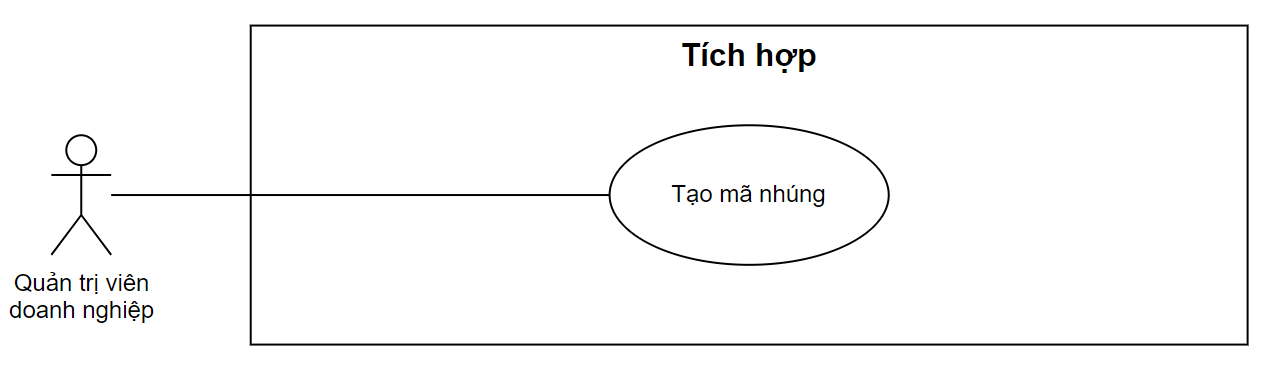
\includegraphics[width=1\linewidth]{Dg_UC/tichhop.png}
    \vspace{0.5cm}
    \caption{Biểu đồ use case cho tích hợp}
    \label{fig:enter-label}
\end{figure}
\subsubsubsection{Usecase scenerio}
\textbf{Tạo mã nhúng}

\begin{table}[H]
\centering
\begin{tabular}{|l|l|l|l|}
\hline
Use case name: & \multicolumn{3}{|l|}{Tạo mã nhúng} \\
\hline
Created by: & Phạm Đức Thắng & Last updated by: & Phạm Đức Thắng \\
\hline
Date created: & 19/10/2024 & Date last updated: & 19/10/2024 \\
\hline
Actors: & \multicolumn{3}{|l|}{Quản trị viên doanh nghiệp} \\
\hline
Description: & \multicolumn{3}{|p{12cm}|}{Quản trị viên doanh nghiệp tạo đoạn mã nhúng và gắn vào website để có thể tích hợp chatbot vào website của họ.} \\
\hline
Trigger: & \multicolumn{3}{|p{12cm}|}{Quản trị viên muốn tạo mã nhúng để tích hợp chatbot vào website.} \\
\hline
Preconditions: & \multicolumn{3}{|p{12cm}|}{
- Quản trị viên đã đăng nhập vào hệ thống. \newline
- Doanh nghiệp đã đăng ký dịch vụ chatbot.
} \\
\hline
Postconditions: & \multicolumn{3}{|p{12cm}|}{Đoạn mã nhúng được tạo thành công và sẵn sàng để tích hợp.} \\
\hline
Normal Flows: & \multicolumn{3}{|p{12cm}|}{
1. Quản trị viên đăng nhập vào hệ thống quản lý chatbot. \newline
2. Điều hướng tới trang “Tùy chỉnh chatbot”. \newline
3. Xem trước kích thước, màu sắc, vị trí hiển thị của chatbot. \newline
4. Nhấn nút "Tạo mã nhúng". \newline
5. Hệ thống tạo và hiển thị đoạn mã nhúng. \newline
6. Quản trị viên sao chép đoạn mã này để gán vào website.
}\\
\hline
Alternative Flows: & \multicolumn{3}{|p{12cm}|}{Không có} \\
\hline
Exceptions: & \multicolumn{3}{|p{12cm}|}{
\textbf{E1: Xảy ra sự cố kỹ thuật trong quá trình tạo đoạn mã nhúng} \newline
5.1. Hệ thống hiển thị thông báo lỗi: "Đã xảy ra lỗi trong quá trình tạo đoạn mã nhúng. Vui lòng thử lại sau."
} \\
\hline
Notes and issues: & \multicolumn{3}{|p{12cm}|}{Không có} \\
\hline
\end{tabular}
\caption{Use case scenario cho Tạo mã nhúng}
\end{table}

%-------------------------------------------------------------------
\subsubsection{Quản lý chatbot}
\subsubsubsection{Biểu đồ use case}
\begin{figure}[H]
    \centering
    % 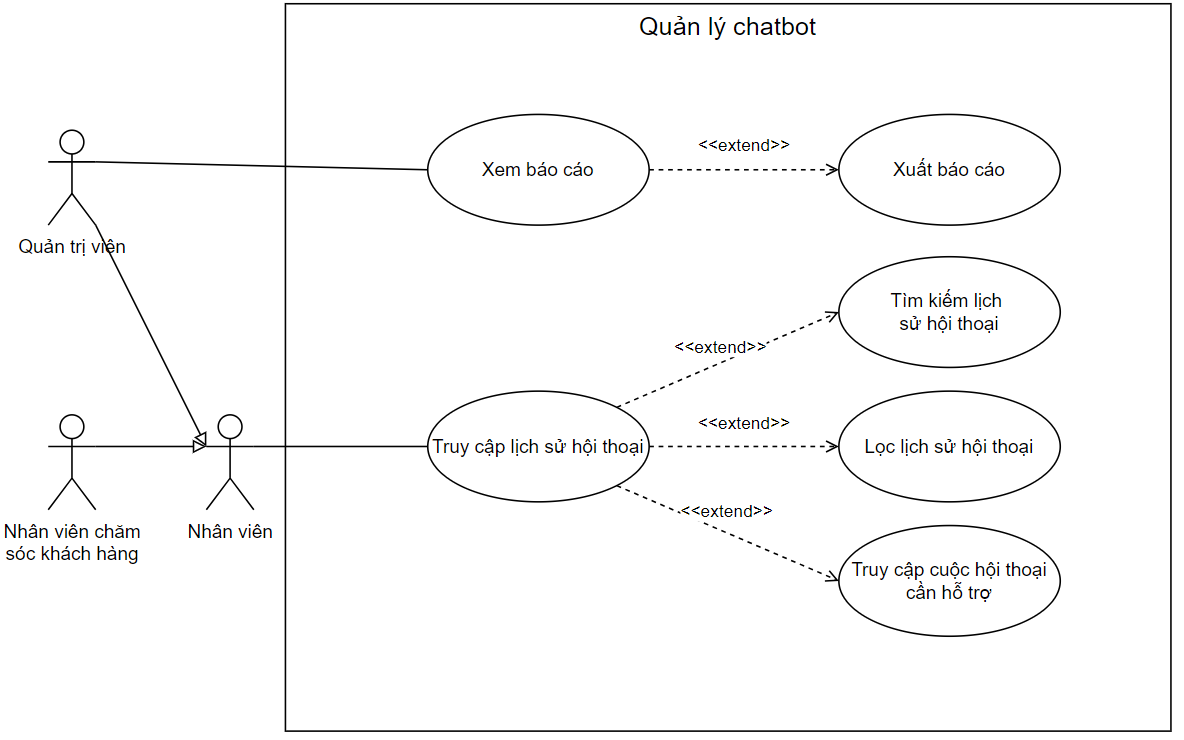
\includegraphics[width=1\linewidth]{Dg_UC/quanlychatbot.png}
    \includesvg[width=1\textwidth]{Dg_UC/Usecase Diagram-ChatbotManagement.drawio.svg}
    \vspace{0.5cm}
    \caption{Biểu đồ use case cho Quản lý chatbot}
    \label{fig:enter-label}
\end{figure}
\subsubsubsection{Use case scenario}
\textbf{Xem báo cáo}
\begin{table}[H]
    \centering
    \begin{tabular}{|l|l|l|l|} 
        \hline
        Use case name: & \multicolumn{3}{|l|}{Xem báo cáo} \\
        \hline
        Created by: & Lê Đình Huy & Last updated by: & Lê Đình Huy \\
        \hline
        Date created: & 19 / 10 / 2024 & Date last updated: & 19 / 10 / 2024 \\
        \hline
        Actors: & \multicolumn{3}{|l|}{Quản trị viên} \\
        \hline
        Description: & \multicolumn{3}{|p{12cm}|}{Cho phép quản trị viên xem báo cáo thống kê về hệ thống chatbot của mình.} \\ 
        \hline
        Trigger: & \multicolumn{3}{|p{12cm}|}{Chọn "Báo cáo" trên thanh điều hướng.} \\
        \hline
        Preconditions: & \multicolumn{3}{|p{12cm}|}{- Quản trị viên có tài khoản trên website. \newline
        - Quản trị viên đã đăng nhập thành công vào hệ thống. \newline
        - Thiết bị của quản trị viên có kết nối mạng và kết nối với hệ thống. \newline
        - Quản trị viên có quyền thực hiện chức năng.} \\
        \hline
        Postconditions: & \multicolumn{3}{|p{12cm}|}{Hệ thống hiển thị các thông số và biểu đồ thống kê.} \\
        \hline
        Normal Flows: & \multicolumn{3}{|p{12cm}|}{1. Quản trị viên chọn "Báo cáo" trên thanh điều hướng. \newline
        2. Hệ thống hiển thị các thông số và báo cáo thống kê.}\\
        \hline
        Alternative Flows: & \multicolumn{3}{|p{12cm}|}{\textbf{A1: Sau bước 2} \newline
        3.1. Quản trị viên chọn "Lọc".\newline
        3.2. Hệ thống hiển thị các thông số cho phép của bộ lọc.\newline
        3.3. Quản trị viên chọn một thông số.\newline
        Tiếp tục bước 2 trong Normal flows.
        } \\
        \hline
        Exceptions: & \multicolumn{3}{|p{12cm}|}{Không có} \\
        \hline
        Note and issues: & \multicolumn{3}{|p{12cm}|}{Không có} \\
        \hline
    \end{tabular}
    \caption{Use case scenario cho Xem báo cáo}
\end{table}

\textbf{Xuất báo cáo}
\begin{table}[H]
    \centering
    \begin{tabular}{|l|l|l|l|} 
        \hline
        Use case name: & \multicolumn{3}{|l|}{Xuất báo cáo} \\
        \hline
        Created by: & Lê Đình Huy & Last updated by: & Lê Đình Huy \\
        \hline
        Date created: & 19 / 10 / 2024 & Date last updated: & 19 / 10 / 2024 \\
        \hline
        Actors: & \multicolumn{3}{|l|}{Quản trị viên} \\
        \hline
        Description: & \multicolumn{3}{|p{12cm}|}{Cho phép quản trị viên xuất báo cáo thống kê về hệ thống chatbot của mình ra file pdf hoặc excel.} \\ 
        \hline
        Trigger: & \multicolumn{3}{|p{12cm}|}{Chọn "Xuất báo cáo" trong giao diện Xem báo cáo.} \\
        \hline
        Preconditions: & \multicolumn{3}{|p{12cm}|}{- Quản trị viên có tài khoản trên website. \newline
        - Quản trị viên đã đăng nhập thành công vào hệ thống. \newline
        - Thiết bị của quản trị viên có kết nối mạng và kết nối với hệ thống. \newline
        - Quản trị viên có quyền thực hiện chức năng.} \\
        \hline
        Postconditions: & \multicolumn{3}{|p{12cm}|}{File báo cáo được tạo và tải về thiết bị của quản trị viên.} \\
        \hline
        Normal Flows: & \multicolumn{3}{|p{12cm}|}{1. Quản trị viên chọn "Xuất báo cáo" trong giao diện Xem báo cáo.\newline
        2. Hệ thống hiển thị hai loại tệp (pdf, excel) cho quản trị viên chọn.\newline
        3. Quản trị viên chọn một loại tệp và chọn "Xem trước".\newline
        4. Hệ thống hiển thị chế độ xem trước file.\newline
        5. Quản trị viên chọn "Tải xuống". \newline
        6. File báo cáo được tải về thiết bị của quản trị viên.}\\
        \hline
        Alternative Flows: & \multicolumn{3}{|p{12cm}|}{Không có} \\
        \hline
        Exceptions: & \multicolumn{3}{|p{12cm}|}{
        \textbf{E1: Tại bước 5} \newline
        5.1. Quản trị viên chọn "Hủy bỏ".\newline
        5.2. Hệ thống đóng chế độ xem trước file.\newline
        Use case dừng lại.
        } \\
        \hline
        Note and issues: & \multicolumn{3}{|p{12cm}|}{Không có} \\
        \hline
    \end{tabular}
    \caption{Use case scenario cho Xem báo cáo}
\end{table}

\textbf{Truy cập lịch sử hội thoại}
\begin{table}[H]
    \centering
    \begin{tabular}{|l|l|l|l|} 
        \hline
        Use case name: & \multicolumn{3}{|l|}{Truy cập lịch sử hội thoại} \\
        \hline
        Created by: & Lê Đình Huy & Last updated by: & Lê Đình Huy \\
        \hline
        Date created: & 19 / 10 / 2024 & Date last updated: & 19 / 10 / 2024 \\
        \hline
        Actors: & \multicolumn{3}{|l|}{Nhân viên} \\
        \hline
        Description: & \multicolumn{3}{|p{12cm}|}{Cho phép nhân viên truy cập và xem lịch sử hội thoại.} \\ 
        \hline
        Trigger: & \multicolumn{3}{|p{12cm}|}{Chọn "Chat" trên thanh điều hướng.} \\
        \hline
        Preconditions: & \multicolumn{3}{|p{12cm}|}{- Nhân viên có tài khoản trên website. \newline
        - Nhân viên đã đăng nhập thành công vào hệ thống. \newline
        - Thiết bị của nhân viên có kết nối mạng và kết nối với hệ thống. \newline
        - Nhân viên có quyền thực hiện chức năng.} \\
        \hline
        Postconditions: & \multicolumn{3}{|p{12cm}|}{Hệ thống hiển thị chi tiết toàn bộ cuộc hội thoại của khách hàng.} \\
        \hline
        Normal Flows: & \multicolumn{3}{|p{12cm}|}{1. Nhân viên chọn "Chat" trên thanh điều hướng.\newline
        2. Hệ thống hiển thị danh sách các cuộc hội thoại.\newline
        3. Nhân viên chọn xem một cuộc hội thoại.\newline
        4. Hệ thống hiển thị chi tiết toàn bộ cuộc hội thoại của khách hàng.}\\
        \hline
        Alternative Flows: & \multicolumn{3}{|p{12cm}|}{
        \textbf{A1: Tại bước 3}\newline
        3.1. Nhân viên chọn vào ô Tìm kiếm và nhập nội dung cần tìm.\newline
        3.2. Nhân viên chọn "Tìm".\newline
        Tiếp tục bước 2 trong Normal flows.\newline
        \textbf{A2: Tại bước 3}\newline
        3.1. Nhân viên chọn "Lọc".\newline
        3.2. Hệ thống hiển thị các thông số cho phép của bộ lọc.\newline
        3.3. Nhân viên chọn một thông số.\newline
        Tiếp tục bước 2 trong Normal flows.\newline
        \textbf{A3: Tại bước 3}\newline
        3.1. Nhân viên chọn "Cần hỗ trợ".\newline
        Tiếp tục bước 2 trong Normal flows.
        } \\
        \hline
        Exceptions: & \multicolumn{3}{|p{12cm}|}{Không có} \\
        \hline
        Note and issues: & \multicolumn{3}{|p{12cm}|}{Không có} \\
        \hline
    \end{tabular}
    \caption{Use case scenario cho Xem báo cáo}
\end{table}

%-------------------------------------------------------------------
\subsubsection{Thông báo và cảnh báo}
\subsubsubsection{Biểu đồ use case}
\begin{figure}[H]
    \centering
    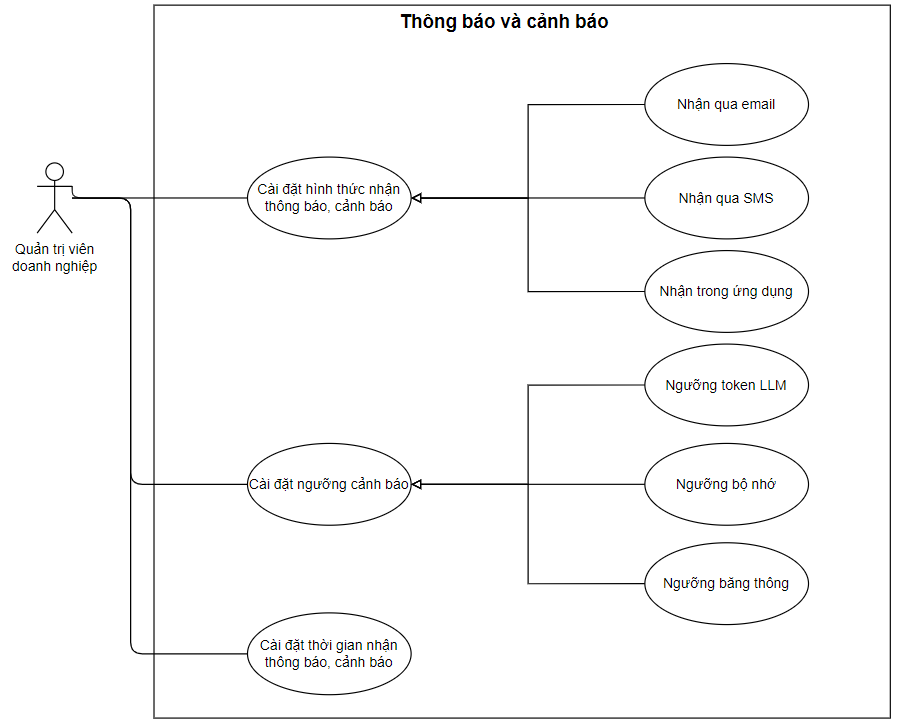
\includegraphics[width=1\linewidth]{Dg_UC/thongbaocanhbao.png}
    \vspace{0.5cm}
    \caption{Biểu đồ use case cho Thông báo và cảnh báo}
    \label{fig:enter-label}
\end{figure}
\subsubsubsection{Use case scenario}

\textbf{Chọn phương thức thông báo và cảnh báo}
\begin{table}[H]
\centering
\begin{tabular}{|l|l|l|l|}
\hline
Use case name: & \multicolumn{3}{|l|}{Chọn phương thức thông báo và cảnh báo} \\
\hline
Created by: & Phạm Đức Thắng & Last updated by: & Phạm Đức Thắng \\
\hline
Date created: & 19/10/2024 & Date last updated: & 19/10/2024 \\
\hline
Actors: & \multicolumn{3}{|l|}{Quản trị viên doanh nghiệp} \\
\hline
Description: & \multicolumn{3}{|p{12cm}|}{Doanh nghiệp có thể chọn cách họ muốn nhận thông báo và cảnh báo liên quan đến hệ thống chatbot.} \\
\hline
Trigger: & \multicolumn{3}{|p{12cm}|}{Quản trị viên muốn thay đổi phương thức nhận thông báo và cảnh báo.} \\
\hline
Preconditions: & \multicolumn{3}{|p{12cm}|}{Người dùng đã đăng nhập vào hệ thống.} \\
\hline
Postconditions: & \multicolumn{3}{|p{12cm}|}{Phương thức thông báo và cảnh báo được lưu và áp dụng cho tài khoản doanh nghiệp.} \\
\hline
Normal Flows: & \multicolumn{3}{|p{12cm}|}{
1. Người dùng truy cập vào trang cài đặt thông báo và cảnh báo. \newline
2. Hệ thống hiển thị các tùy chọn phương thức. \newline
3. Người dùng chọn hoặc hủy chọn các phương thức nhận thông báo: email và trong ứng dụng. \newline
4. Người dùng xác nhận lựa chọn. \newline
5. Hệ thống lưu cài đặt và hiển thị thông báo xác nhận.
}\\
\hline
Alternative Flows: & \multicolumn{3}{|p{12cm}|}{Không có} \\
\hline
Exceptions: & \multicolumn{3}{|p{12cm}|}{
\textbf{E1. Hệ thống không thể lưu cài đặt} \newline
5.1. Hệ thống hiển thị thông báo lỗi. \newline
5.2. Người dùng có thể thử lại hoặc hủy bỏ thao tác.
} \\
\hline
Notes and issues: & \multicolumn{3}{|p{12cm}|}{Không có} \\
\hline
\end{tabular}
\caption{Use case scenario cho Chọn phương thức thông báo và cảnh báo}
\end{table}

\textbf{Thiết lập ngưỡng cảnh báo}

\begin{table}[H]
\centering
\begin{tabular}{|l|l|l|l|}
\hline
Use case name: & \multicolumn{3}{|l|}{Thiết lập ngưỡng cảnh báo} \\
\hline
Created by: & Phạm Đức Thắng & Last updated by: & Phạm Đức Thắng \\
\hline
Date created: & 19/10/2024 & Date last updated: & 19/10/2024 \\
\hline
Actors: & \multicolumn{3}{|l|}{Quản trị viên doanh nghiệp} \\
\hline
Description: & \multicolumn{3}{|p{12cm}|}{Doanh nghiệp có thể thiết lập ngưỡng cảnh báo cho việc sử dụng token LLM và lưu lượng truy cập.} \\
\hline
Trigger: & \multicolumn{3}{|p{12cm}|}{Quản trị viên muốn thay đổi ngưỡng cảnh báo cho việc sử dụng token LLM và lưu lượng truy cập.} \\
\hline
Preconditions: & \multicolumn{3}{|p{12cm}|}{Người dùng đã đăng nhập vào hệ thống.} \\
\hline
Postconditions: & \multicolumn{3}{|p{12cm}|}{Ngưỡng cảnh báo được lưu và áp dụng cho tài khoản người dùng.} \\
\hline
Normal Flows: & \multicolumn{3}{|p{12cm}|}{
1. Người dùng truy cập vào trang cài đặt thông báo và cảnh báo. \newline
2. Hệ thống hiển thị các tùy chọn ngưỡng. \newline
3. Người dùng thiết lập ngưỡng cảnh báo cho việc sử dụng token LLM. \newline
4. Người dùng thiết lập ngưỡng cảnh báo cho lưu lượng truy cập. \newline
5. Người dùng xác nhận các cài đặt. \newline
6. Hệ thống lưu cài đặt và hiển thị thông báo xác nhận.
}\\
\hline
Alternative Flows: & \multicolumn{3}{|p{12cm}|}{
\textbf{A1. Người dùng tắt cảnh báo cho việc sử dụng token LLM} \newline
3.1. Người dùng bấm nút tắt cảnh báo cho việc sử dụng token LLM \newline
\textbf{A2. Người dùng tắt cảnh báo cho lưu lượng truy cập} \newline
4.1. Người dùng bấm nút tắt cảnh báo cho lưu lượng truy cập
} \\
\hline
Exceptions: & \multicolumn{3}{|p{12cm}|}{
\textbf{E1. Hệ thống không thể lưu cài đặt} \newline
6.1. Hệ thống hiển thị thông báo lỗi. \newline
6.2. Người dùng có thể thử lại hoặc hủy bỏ thao tác.
} \\
\hline
Notes and issues: & \multicolumn{3}{|p{12cm}|}{Không có} \\
\hline
\end{tabular}
\caption{Use case scenario cho Thiết lập ngưỡng cảnh báo}
\end{table}

%-------------------------------------------------------------------
\subsubsection{Quản lý thanh toán}
\subsubsubsection{Biểu đồ usecase}
\begin{figure}[H]
    \centering
    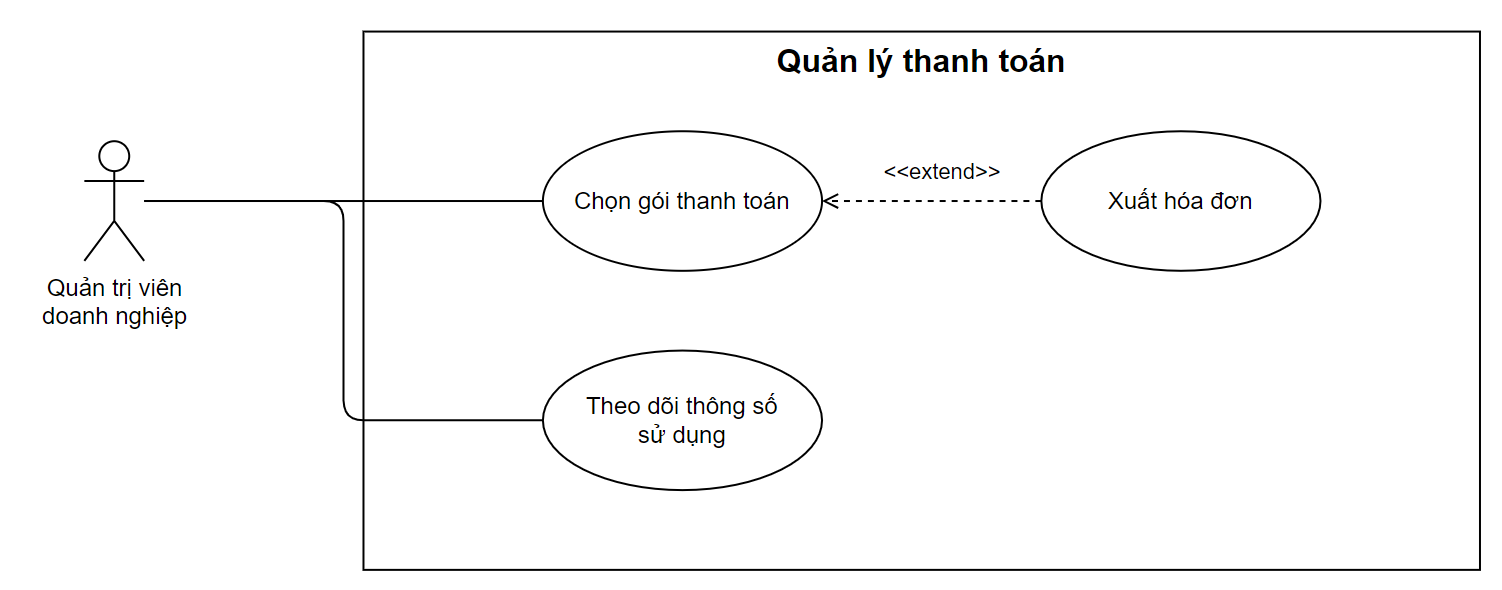
\includegraphics[width=1\linewidth]{Dg_UC/quanlythanhtoan.png}
    \vspace{0.5cm}
    \caption{Biểu đồ use case cho Quản lý thanh toán}
    \label{fig:enter-label}
\end{figure}
\subsubsubsection{Usecase scenerio}
\textbf{Chọn gói thanh toán}

\begin{table}[H]
\centering
\begin{tabular}{|l|l|l|l|}
\hline
Use case name: & \multicolumn{3}{|l|}{Chọn gói thanh toán} \\
\hline
Created by: & Phạm Đức Thắng & Last updated by: & Phạm Đức Thắng \\
\hline
Date created: & 19/10/2024 & Date last updated: & 19/10/2024 \\
\hline
Actors: & \multicolumn{3}{|l|}{Doanh nghiệp} \\
\hline
Description: & \multicolumn{3}{|p{12cm}|}{Doanh nghiệp lựa chọn gói đăng ký phù hợp với nhu cầu sử dụng dịch vụ chatbot từ các gói có sẵn trên hệ thống.} \\
\hline
Trigger: & \multicolumn{3}{|p{12cm}|}{Doanh nghiệp muốn chọn hoặc thay đổi gói đăng ký dịch vụ chatbot.} \\
\hline
Preconditions: & \multicolumn{3}{|p{12cm}|}{
- Doanh nghiệp đã đăng ký và đăng nhập vào tài khoản của mình trên hệ thống. \newline
- Hệ thống đã có các gói đăng ký được cấu hình sẵn.
} \\
\hline
Postconditions: & \multicolumn{3}{|p{12cm}|}{
- Doanh nghiệp đã chọn và xác nhận gói đăng ký mới. \newline
- Hệ thống đã cập nhật gói đăng ký của doanh nghiệp và thực hiện thanh toán nếu cần.
} \\
\hline
Normal Flows: & \multicolumn{3}{|p{12cm}|}{
1. Doanh nghiệp đăng nhập vào tài khoản của mình trên trang web hoặc ứng dụng. \newline
2. Doanh nghiệp điều hướng vào trang "Gói đăng ký". \newline
3. Hệ thống hiển thị danh sách các gói đăng ký hiện có với các tính năng và giá cả tương ứng. \newline
4. Doanh nghiệp chọn gói đăng ký mong muốn bằng cách nhấp vào nút "Mua". \newline
5. Hệ thống hiển thị thông tin chi tiết của gói đăng ký đã chọn và yêu cầu xác nhận. \newline
6. Doanh nghiệp xác nhận lựa chọn và tiến hành thanh toán. \newline
7. Hệ thống xử lý giao dịch thanh toán và cập nhật trạng thái gói đăng ký cho doanh nghiệp. \newline
8. Hệ thống hiển thị thông báo xác nhận thành công.
}\\
\hline
Alternative Flows: & \multicolumn{3}{|p{12cm}|}{
\textbf{A1: Thay đổi gói đăng ký} \newline
4.1. Doanh nghiệp chọn gói đăng ký mới muốn nâng cấp hoặc giảm cấp. \newline
4.2. Hệ thống tính toán sự khác biệt về giá cả. \newline
4.3. Doanh nghiệp xác nhận lựa chọn và tiến hành thanh toán nếu cần. \newline
4.4. Hệ thống cập nhật gói đăng ký mới cho doanh nghiệp và điều chỉnh các dịch vụ liên quan. \newline\newline
\textbf{A2: Doanh nghiệp chọn xuất hóa đơn} \newline
6.1. Sau khi thanh toán thành công, hệ thống cung cấp tùy chọn "Xuất Hóa Đơn". \newline
6.2. Doanh nghiệp chọn "Xuất Hóa Đơn" để tải xuống hóa đơn hoặc gửi qua email. \newline
6.3. Hệ thống tạo và gửi hóa đơn đến email đã đăng ký. \newline
6.4. Doanh nghiệp nhận được hóa đơn để lưu trữ và quản lý chi tiêu.
} \\
\hline
Exceptions: & \multicolumn{3}{|p{12cm}|}{
\textbf{E1 Giao dịch thanh toán không thành công do lỗi thẻ tín dụng, thiếu tiền trong tài khoản hoặc sự cố mạng.} \newline
7.1. Khi doanh nghiệp cố gắng thanh toán, hệ thống kiểm tra và phát hiện lỗi. \newline
7.2. Hệ thống hiển thị thông báo lỗi: "Thanh toán không thành công. Vui lòng kiểm tra thông tin thanh toán hoặc thử lại sau." \newline
7.3. Doanh nghiệp có thể thử lại giao dịch hoặc thay đổi thông tin thanh toán khác.
} \\
\hline
Notes and issues: & \multicolumn{3}{|p{12cm}|}{Không có} \\
\hline
\end{tabular}
\caption{Use case scenario cho Chọn gói thanh toán}
\end{table}

\textbf{Theo dõi thông số sử dụng}

\begin{table}[H]
\centering
\begin{tabular}{|l|l|l|l|}
\hline
Use case name: & \multicolumn{3}{|l|}{Theo dõi thông số sử dụng} \\
\hline
Created by: & Phạm Đức Thắng & Last updated by: & Phạm Đức Thắng \\
\hline
Date created: & 19/10/2024 & Date last updated: & 19/10/2024 \\
\hline
Actors: & \multicolumn{3}{|l|}{Doanh nghiệp} \\
\hline
Description: & \multicolumn{3}{|p{12cm}|}{Doanh nghiệp có thể theo dõi các thông số giới han của gói đã đăng ký, bao gồm thời hạn gói đăng ký, số lượng yêu cầu và bộ nhớ đã sử dụng.} \\
\hline
Trigger: & \multicolumn{3}{|p{12cm}|}{Doanh nghiệp muốn xem thông tin về mức độ sử dụng dịch vụ chatbot.} \\
\hline
Preconditions: & \multicolumn{3}{|p{12cm}|}{
- Doanh nghiệp đã đăng ký và sử dụng dịch vụ chatbot. \newline
- Hệ thống đã ghi nhận dữ liệu sử dụng dịch vụ của doanh nghiệp.
} \\
\hline
Postconditions: & \multicolumn{3}{|p{12cm}|}{Doanh nghiệp đã xem được các thông số sử dụng dịch vụ chi tiết.} \\
\hline
Normal Flows: & \multicolumn{3}{|p{12cm}|}{
1. Doanh nghiệp đăng nhập vào tài khoản của mình. \newline
2. Doanh nghiệp truy cập vào trang "Quản lý thanh toán". \newline
3. Hệ thống hiển thị các thông số sử dụng hiện tại như số lượng yêu cầu đã xử lý, thời gian gói còn lại và bộ nhớ đã sử dụng.
}\\
\hline
Alternative Flows: & \multicolumn{3}{|p{12cm}|}{Không có} \\
\hline
Exceptions: & \multicolumn{3}{|p{12cm}|}{
\textbf{E1: Hệ thống chưa có dữ liệu sử dụng do mới bắt đầu dịch vụ hoặc vấn đề kỹ thuật} \newline
5.1. Hệ thống kiểm tra và phát hiện thiếu dữ liệu. \newline
5.2. Hiển thị thông báo: "Chưa có dữ liệu sử dụng để hiển thị. Vui lòng quay lại sau."
} \\
\hline
Notes and issues: & \multicolumn{3}{|p{12cm}|}{Không có} \\
\hline
\end{tabular}
\caption{Use case scenario cho Theo dõi sử dụng}
\end{table}

%-------------------------------------------------------------------
\subsubsection{Tương tác với chatbot}
\subsubsubsection{Biểu đồ use case}
\begin{figure}[H]
    \centering
    % 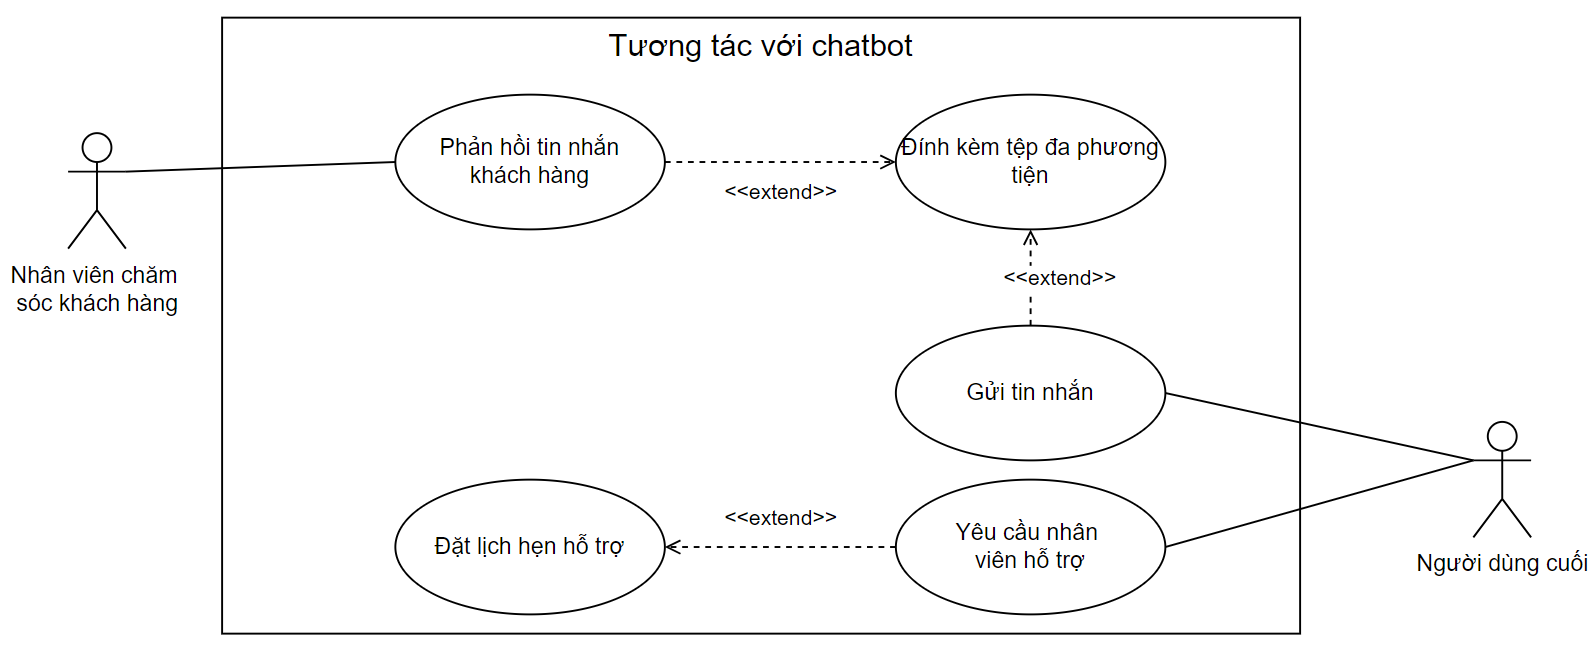
\includegraphics[width=1\linewidth]{Dg_UC/tuongtacvoichatbot.png}
    \includesvg[width=1\textwidth]{Dg_UC/Usecase Diagram-ChatbotInteraction.drawio.svg}
    \vspace{0.5cm}
    \caption{Biểu đồ use case cho Tương tác với chatbot}
    \label{fig:enter-label}
\end{figure}
\subsubsubsection{Use case scenario}
\textbf{Phản hồi tin nhắn khách hàng}
\begin{table}[H]
    \centering
    \begin{tabular}{|l|l|l|l|} 
        \hline
        Use case name: & \multicolumn{3}{|l|}{Phản hồi tin nhắn khách hàng} \\
        \hline
        Created by: & Lê Đình Huy & Last updated by: & Lê Đình Huy \\
        \hline
        Date created: & 19 / 10 / 2024 & Date last updated: & 19 / 10 / 2024 \\
        \hline
        Actors: & \multicolumn{3}{|l|}{Nhân viên chăm sóc khách hàng} \\
        \hline
        Description: & \multicolumn{3}{|p{12cm}|}{Cho phép nhân viên chăm sóc khách hàng phản hồi trực tiếp tin nhắn của khách hàng.} \\ 
        \hline
        Trigger: & \multicolumn{3}{|p{12cm}|}{Chọn vào xem đoạn hội thoại với một khách hàng.} \\
        \hline
        Preconditions: & \multicolumn{3}{|p{12cm}|}{- Nhân viên có tài khoản trên website. \newline
        - Nhân viên đã đăng nhập thành công vào hệ thống. \newline
        - Thiết bị của nhân viên có kết nối mạng và kết nối với hệ thống. \newline
        - Nhân viên có quyền thực hiện chức năng.} \\
        \hline
        Postconditions: & \multicolumn{3}{|p{12cm}|}{Tin nhắn được gửi thành công và hiển thị ở hai phía.} \\
        \hline
        Normal Flows: & \multicolumn{3}{|p{12cm}|}{1. Nhân viên CSKH chọn vào xem đoạn hội thoại với một khách hàng. \newline
        2. Hệ thống hiển thị màn hình chat với khách hàng đó. \newline
        3. Nhân viên CSKH chọn vào khung điền tin nhắn và nhập nội dung tin nhắn. \newline
        4. Nhân viên CSKH chọn "Gửi". \newline
        5. Hệ thống lưu dữ liệu vào database và hiển thị tin nhắn vừa gửi lên màn hình.} \\
        \hline
        Alternative Flows: & \multicolumn{3}{|p{12cm}|}{\textbf{A1: Tại bước 3 hoặc 4} \newline
        Khi nhân viên CSKH muốn đính kèm tệp, chuyển đến use case Đính kèm tệp đa phương tiện. Sau đó tiếp tục tại bước đó trong Normal flows.} \\
        \hline
        Exceptions: & \multicolumn{3}{|p{12cm}|}{Không có} \\
        \hline
        Note and issues: & \multicolumn{3}{|p{12cm}|}{Không có} \\
        \hline
    \end{tabular}
    \caption{Use case scenario cho Phản hồi tin nhắn khách hàng}
\end{table}

\textbf{Gửi tin nhắn}
\begin{table}[H]
    \centering
    \begin{tabular}{|l|l|l|l|} 
        \hline
        Use case name: & \multicolumn{3}{|l|}{Gửi tin nhắn} \\
        \hline
        Created by: & Lê Đình Huy & Last updated by: & Lê Đình Huy \\
        \hline
        Date created: & 19 / 10 / 2024 & Date last updated: & 19 / 10 / 2024 \\
        \hline
        Actors: & \multicolumn{3}{|l|}{Người dùng cuối (Khách hàng)} \\
        \hline
        Description: & \multicolumn{3}{|p{12cm}|}{Cho phép người dùng cuối gửi tin nhắn trong chatbot.} \\ 
        \hline
        Trigger: & \multicolumn{3}{|p{12cm}|}{Chọn vào nút chatbot trên website của doanh nghiệp.} \\
        \hline
        Preconditions: & \multicolumn{3}{|p{12cm}|}{- Thiết bị của người dùng có kết nối mạng.} \\
        \hline
        Postconditions: & \multicolumn{3}{|p{12cm}|}{Tin nhắn được gửi thành công và hiển thị trên màn hình. \newline
        Đồng thời, tin nhắn từ chatbot sẽ phản hồi lại trong một khoảng thời gian nhất định.} \\
        \hline
        Normal Flows: & \multicolumn{3}{|p{12cm}|}{1. Người dùng chọn vào nút chatbot trên website của doanh nghiệp. \newline
        2. Hệ thống hiển thị màn hình chatbot. \newline
        3. Người dùng chọn vào khung điền tin nhắn và nhập nội dung tin nhắn. \newline
        4. Người dùng chọn "Gửi". \newline
        5. Hệ thống lưu dữ liệu vào database và hiển thị tin nhắn vừa gửi lên màn hình. \newline
        6. Hệ thống chatbot tạo và phản hồi người dùng trong một khoảng thời gian nhất định.} \\
        \hline
        Alternative Flows: & \multicolumn{3}{|p{12cm}|}{\textbf{A1: Tại bước 3 hoặc 4} \newline
        Khi người dùng muốn đính kèm tệp, chuyển đến use case Đính kèm tệp đa phương tiện. Sau đó tiếp tục tại bước đó trong Normal flows.} \\
        \hline
        Exceptions: & \multicolumn{3}{|p{12cm}|}{Không có} \\
        \hline
        Note and issues: & \multicolumn{3}{|p{12cm}|}{Không có} \\
        \hline
    \end{tabular}
    \caption{Use case scenario cho Gửi tin nhắn}
\end{table}


\textbf{Đính kèm tệp đa phương tiện}
\begin{table}[H]
    \centering
    \begin{tabular}{|l|l|l|l|} 
        \hline
        Use case name: & \multicolumn{3}{|l|}{Đính kèm tệp đa phương tiện} \\
        \hline
        Created by: & Lê Đình Huy & Last updated by: & Lê Đình Huy \\
        \hline
        Date created: & 19 / 10 / 2024 & Date last updated: & 19 / 10 / 2024 \\
        \hline
        Actors: & \multicolumn{3}{|l|}{Nhân viên CSKH, người dùng cuối (Khách hàng)} \\
        \hline
        Description: & \multicolumn{3}{|p{12cm}|}{Cho phép nhân viên CSKH và người dùng cuối đính kèm tệp đa phương tiện.} \\ 
        \hline
        Trigger: & \multicolumn{3}{|p{12cm}|}{Chọn vào nút "Đính kèm tệp đa phương tiện" trong khung chat.} \\
        \hline
        Preconditions: & \multicolumn{3}{|p{12cm}|}{Preconditions của tính năng Phản hồi tin nhắn khách hàng đối với nhân viên CSKH, tính năng Gửi tin nhắn đối với người dùng cuối.} \\
        \hline
        Postconditions: & \multicolumn{3}{|p{12cm}|}{Hệ thống hiển thị ảnh được chọn lên màn hình.} \\
        \hline
        Normal Flows: & \multicolumn{3}{|p{12cm}|}{1. Người dùng chọn vào nút "Đính kèm tệp đa phương tiện". \newline
        2. Hệ thống hiển thị màn hình chọn ảnh. \newline
        3. Người dùng chọn một bức ảnh trên thiết bị. \newline
        4. Người dùng chọn "Tải lên". \newline
        5. Hệ thống hiển thị ảnh được chọn lên màn hình.} \\
        \hline
        Alternative Flows: & \multicolumn{3}{|p{12cm}|}{Không có} \\
        \hline
        Exceptions: & \multicolumn{3}{|p{12cm}|}{\textbf{E1: Sau bước 5} \newline
        6.1. Người dùng chọn nút "Xóa" ảnh vừa tải. \newline
        6.2. Ảnh vừa tải bị xóa khỏi màn hình. \newline
        Use case dừng lại.} \\
        \hline
        Note and issues: & \multicolumn{3}{|p{12cm}|}{Không có} \\
        \hline
    \end{tabular}
    \caption{Use case scenario cho Đính kèm tệp đa phương tiện}
\end{table}


\textbf{Yêu cầu nhân viên hỗ trợ}
\begin{table}[H]
    \centering
    \begin{tabular}{|l|l|l|l|} 
        \hline
        Use case name: & \multicolumn{3}{|l|}{Yêu cầu nhân viên hỗ trợ} \\
        \hline
        Created by: & Lê Đình Huy & Last updated by: & Lê Đình Huy \\
        \hline
        Date created: & 19 / 10 / 2024 & Date last updated: & 19 / 10 / 2024 \\
        \hline
        Actors: & \multicolumn{3}{|l|}{Người dùng cuối (Khách hàng)} \\
        \hline
        Description: & \multicolumn{3}{|p{12cm}|}{Cho phép người dùng cuối có thể yêu cầu nhân viên hỗ trợ.} \\ 
        \hline
        Trigger: & \multicolumn{3}{|p{12cm}|}{Chọn vào nút yêu cầu hỗ trợ trong khung chatbot.} \\
        \hline
        Preconditions: & \multicolumn{3}{|p{12cm}|}{- Thiết bị của người dùng có kết nối mạng.} \\
        \hline
        Postconditions: & \multicolumn{3}{|p{12cm}|}{Yêu cầu được gửi lên hệ thống và màn hình hiển thị thông báo thành công. Đồng thời, tính năng chat tự động sẽ được tạm dừng.} \\
        \hline
        Normal Flows: & \multicolumn{3}{|p{12cm}|}{1. Người dùng chọn vào nút yêu cầu hỗ trợ trong khung chatbot. \newline
        2. Hệ thống hiển thị pop up Hỗ trợ khách hàng. \newline
        3. Người dùng chọn "Gửi yêu cầu". \newline
        4. Yêu cầu được gửi lên hệ thống và màn hình hiển thị thông báo thành công. Đồng thời, tính năng chat tự động sẽ được tạm dừng.} \\
        \hline
        Alternative Flows: & \multicolumn{3}{|p{12cm}|}{Không có} \\
        \hline
        Exceptions: & \multicolumn{3}{|p{12cm}|}{\textbf{E1: Tại bước 3} \newline
        3.1. Người dùng chọn "Đặt lịch hẹn". \newline
        Chuyển đến use case Đặt lịch hẹn hỗ trợ. Use case dừng lại. \newline
        \textbf{E2: Tại bước 3} \newline
        3.1. Người dùng chọn "Đóng". \newline
        3.2. Pop up Hỗ trợ khách hàng được đóng. \newline
        Use case dừng lại.} \\
        \hline
        Note and issues: & \multicolumn{3}{|p{12cm}|}{Không có} \\
        \hline
    \end{tabular}
    \caption{Use case scenario cho Yêu cầu nhân viên hỗ trợ}
\end{table}


\textbf{Đặt lịch hẹn hỗ trợ}
\begin{table}[H]
    \centering
    \begin{tabular}{|l|l|l|l|} 
        \hline
        Use case name: & \multicolumn{3}{|l|}{Đặt lịch hẹn hỗ trợ} \\
        \hline
        Created by: & Lê Đình Huy & Last updated by: & Lê Đình Huy \\
        \hline
        Date created: & 19 / 10 / 2024 & Date last updated: & 19 / 10 / 2024 \\
        \hline
        Actors: & \multicolumn{3}{|l|}{Người dùng cuối (Khách hàng)} \\
        \hline
        Description: & \multicolumn{3}{|p{12cm}|}{Cho phép người dùng cuối có thể đặt lịch hẹn hỗ trợ theo thời gian mình mong muốn.} \\ 
        \hline
        Trigger: & \multicolumn{3}{|p{12cm}|}{Chọn vào nút "Đặt lịch hẹn" trong pop up Hỗ trợ khách hàng.} \\
        \hline
        Preconditions: & \multicolumn{3}{|p{12cm}|}{- Thiết bị của người dùng có kết nối mạng.} \\
        \hline
        Postconditions: & \multicolumn{3}{|p{12cm}|}{Lịch hẹn được gửi lên hệ thống và màn hình hiển thị thông báo thành công.} \\
        \hline
        Normal Flows: & \multicolumn{3}{|p{12cm}|}{1. Người dùng chọn vào nút "Đặt lịch hẹn" trong pop up Hỗ trợ khách hàng. \newline
        2. Hệ thống đóng pop up Hỗ trợ khách hàng và hiển thị pop up Đặt lịch hẹn. \newline
        3. Người dùng điền đầy đủ thông tin (tên, số điện thoại, lời nhắn) và chọn lịch có sẵn. \newline
        4. Người dùng chọn "Gửi". \newline
        5. Lịch hẹn được gửi lên hệ thống và màn hình hiển thị thông báo thành công.} \\
        \hline
        Alternative Flows: & \multicolumn{3}{|p{12cm}|}{Không có} \\
        \hline
        Exceptions: & \multicolumn{3}{|p{12cm}|}{\textbf{E1: Tại bước 3 hoặc 4} \newline
        3.1. Người dùng chọn "Đóng". \newline
        3.2. Pop up Đặt lịch hẹn được đóng. \newline
        Use case dừng lại.} \\
        \hline
        Note and issues: & \multicolumn{3}{|p{12cm}|}{Không có} \\
        \hline
    \end{tabular}
    \caption{Use case scenario cho Đặt lịch hẹn hỗ trợ}
\end{table}

%-------------------------------------------------------------------
\subsubsection{Quản lý lịch hẹn}
\subsubsubsection{Biểu đồ use case}
\begin{figure}[H]
    \centering
    % 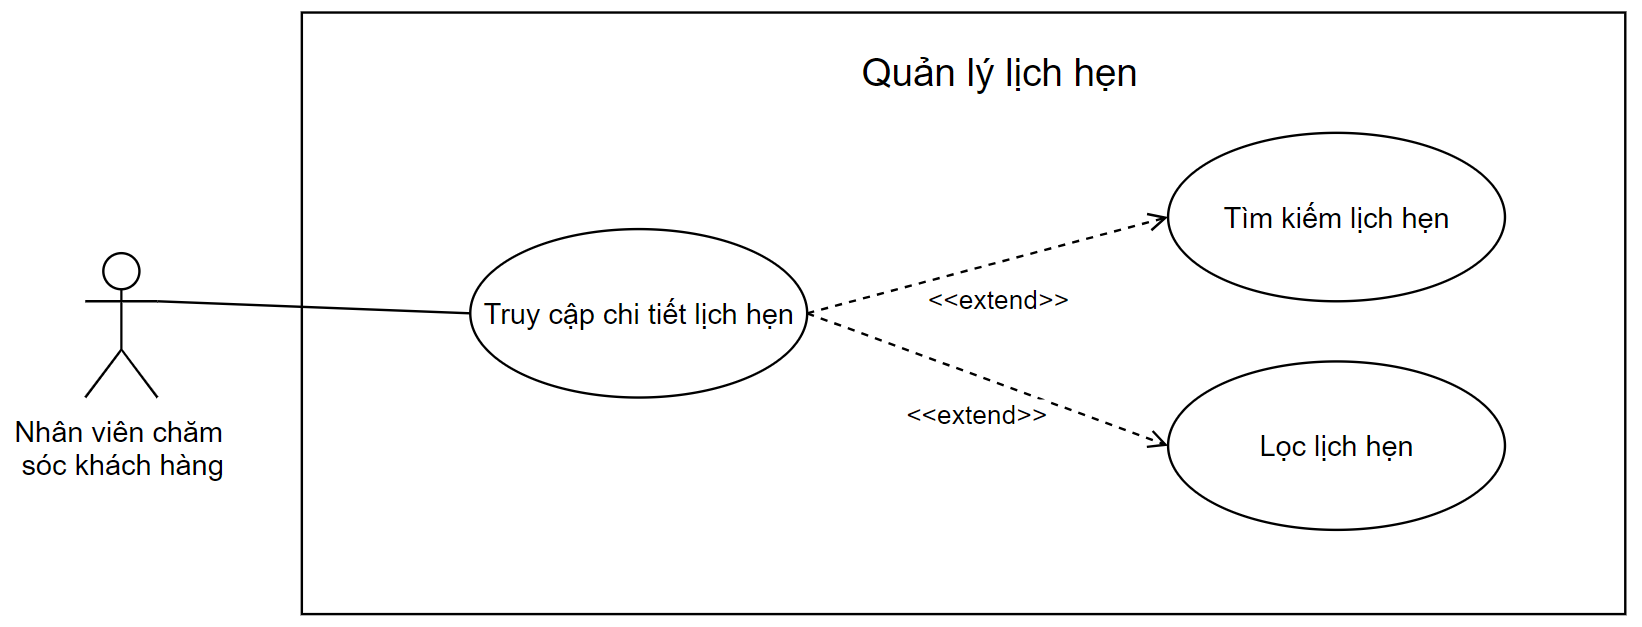
\includegraphics[width=1\linewidth]{Dg_UC/quanlylichhen.png}
    \includesvg[width=1\textwidth]{Dg_UC/Usecase Diagram-AppointmentManagement.drawio.svg}
    \vspace{0.5cm}
    \caption{Biểu đồ use case cho Quản lý lịch hẹn}
    \label{fig:enter-label}
\end{figure}
\subsubsubsection{Use case scenario}
\textbf{Truy cập chi tiết lịch hẹn}
\begin{table}[H]
    \centering
    \begin{tabular}{|l|l|l|l|} 
        \hline
        Use case name: & \multicolumn{3}{|l|}{Truy cập chi tiết lịch hẹn} \\
        \hline
        Created by: & Lê Đình Huy & Last updated by: & Lê Đình Huy \\
        \hline
        Date created: & 19 / 10 / 2024 & Date last updated: & 19 / 10 / 2024 \\
        \hline
        Actors: & \multicolumn{3}{|l|}{Nhân viên chăm sóc khách hàng} \\
        \hline
        Description: & \multicolumn{3}{|p{12cm}|}{Cho phép nhân viên CSKH truy cập và xem chi tiết lịch hẹn.} \\ 
        \hline
        Trigger: & \multicolumn{3}{|p{12cm}|}{Chọn "Lịch hẹn" trên thanh điều hướng.} \\
        \hline
        Preconditions: & \multicolumn{3}{|p{12cm}|}{- Nhân viên có tài khoản trên website. \newline
        - Nhân viên đã đăng nhập thành công vào hệ thống. \newline
        - Thiết bị của nhân viên có kết nối mạng và kết nối với hệ thống. \newline
        - Nhân viên có quyền thực hiện chức năng.} \\
        \hline
        Postconditions: & \multicolumn{3}{|p{12cm}|}{Hệ thống hiển thị chi tiết thông tin lịch hẹn mà khách hàng đã đặt.} \\
        \hline
        Normal Flows: & \multicolumn{3}{|p{12cm}|}{1. Nhân viên CSKH chọn "Lịch hẹn" trên thanh điều hướng.\newline
        2. Hệ thống hiển thị danh sách các lịch hẹn.\newline
        3. Nhân viên CSKH chọn xem một lịch hẹn.\newline
        4. Hệ thống hiển thị chi tiết thông tin lịch hẹn mà khách hàng đã đặt.}\\
        \hline
        Alternative Flows: & \multicolumn{3}{|p{12cm}|}{
        \textbf{A1: Tại bước 3}\newline
        3.1. Nhân viên CSKH chọn vào ô Tìm kiếm và nhập nội dung cần tìm.\newline
        3.2. Nhân viên CSKH chọn "Tìm".\newline
        Tiếp tục bước 2 trong Normal flows.\newline
        \textbf{A2: Tại bước 3}\newline
        3.1. Nhân viên CSKH chọn "Lọc".\newline
        3.2. Hệ thống hiển thị các thông số cho phép của bộ lọc.\newline
        3.3. Nhân viên CSKH chọn một thông số.\newline
        Tiếp tục bước 2 trong Normal flows.} \\
        \hline
        Exceptions: & \multicolumn{3}{|p{12cm}|}{
        \textbf{E1: Tại bước 3 hoặc sau bước 4}\newline
        3.1. Nhân viên CSKH chọn "Hỗ trợ".\newline
        3.2. Hệ thống chuyển đến trang hội thoại với khách hàng.\newline
        Use case dừng lại.
        } \\
        \hline
        Note and issues: & \multicolumn{3}{|p{12cm}|}{Không có} \\
        \hline
    \end{tabular}
    \caption{Use case scenario cho Truy cập chi tiết lịch hẹn}
\end{table}

%-------------------------------------------------------------------
